\documentclass[a4paper]{article}

%% Language and font encodings
%\usepackage[english]{babel}
\usepackage[spanish]{babel}
\usepackage[utf8x]{inputenc}
\usepackage[T1]{fontenc}

%% Sets page size and margins
\usepackage[a4paper,top=3cm,bottom=2cm,left=3cm,right=3cm,marginparwidth=1.75cm]{geometry}

%% Useful packages
\usepackage{amsmath}
\usepackage{graphicx}
\usepackage[colorinlistoftodos]{todonotes}
\usepackage[colorlinks=true, allcolors=blue]{hyperref}

\title{Procesamiento digital de señales de audio - Hoja 4}
\author{Julieta Umpierrez}
\date{\vspace{-5ex}}
\begin{document}
\maketitle

\section{Ejercicio 1 }
En este ejercicio se estudia el cepstrum de señales de audio.
\subsection{Parte 1}
\subsubsection{1}
En esta parte se calcula el cepstrum complejo de un tren de pulsos periódicos. El tren de pulsos periódicos se modela como 
$$p[n]=\beta^n\sum_{k=0}^{\infty}\delta[n-kP]$$
Por definición, el cepstrum complejo es 
$$\hat{p}[n] = \frac{1}{2\pi} \int^{\pi}_{-\pi}log(P(e^{jw}))e^{jwn}dw$$
En primer lugar se calcula $P(e^{jw})$. Para eso se calcula la transformada z de p[n]. 
$$P(z) = \sum_{n=-\infty}^{+\infty}\beta^n\sum_{k=0}^{+\infty}\delta[n-kP]z^{-n}=\sum_{n=-\infty}^{+\infty}\sum_{k=0}^{+\infty}\delta[n-kp]\bigg(\frac{\beta}{z}\bigg)^{kP} = \sum_{k=0}^{+\infty} \bigg(\frac{\beta^P}{z^P}\bigg)^k = \frac{1}{1-(\beta z^{-1})^P}$$
El siguiente paso es tomar el logaritmo e identificar una serie de potencias
$$-log(1-(\beta z^{-1})^P) = \sum_{n=1}^{+\infty}\frac{\beta^{nP}}{n}(z)^{-nP} \overbrace{=}^{(1)}P\sum_{n=1}^{+\infty}\frac{\beta^{nP}}{nP}(z^P)^{-n} \overbrace{=}^{(2)} \sum_{n=1}^{+\infty}\bigg(P\sum_{k=1}^{+\infty} \delta[n-kP] \frac{\beta^{n}}{n}\bigg)z^{-n}$$
donde $(1)$ es multiplicando y dividiendo por $P$ para que se forme $nP$ en el denominador y $(2)$ es escribiéndolo como un peine y utilizando que la sumatoria es la misma tanto en $n$ como en $k$. Luego se identifica que se tiene, por definición la transformada Z de la señal asociada a lo que esta dentro de los paréntesis. Dado que se tiene que el siguiente paso es antitransformar, se tiene que 
$$\hat{p}[n] = P\sum_{k=1}^{+\infty} \delta[n-kP] \frac{\beta^{n}}{n}$$
donde dado que no se esta sumando en $n$ se puede escribir como 
$$\hat{p}[n] = P\frac{\beta^{n}}{n}\sum_{k=1}^{+\infty} \delta[n-kP] $$

En la figura \ref{phatp} se adjuntan las gráficas de la señal original y del cepstrum complejo.
\begin{figure}[h!]
\centering
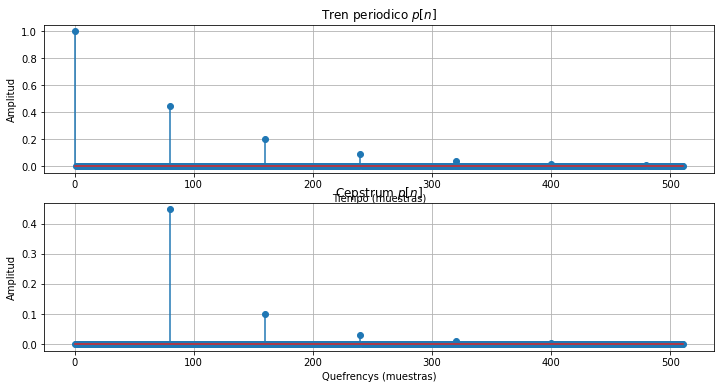
\includegraphics[width=0.8\textwidth]{cepstrum1.png}
\caption{Graficas de $p[n]$ y $\hat{p}[n]$}
\label{phatp}
\end{figure}

\subsubsection{2}
En esta parte se intenta calcular el cepstrum complejo de la señal con la siguiente transformada Z
$$ H(z) = \frac{(1-bz)(1-b^*z)}{(1-cz^{-1})(1-c^*z^{-1})}$$
para esto se va aplicar el mismo procedimiento que la parte anterior pero desde el paso siguiente a obtener la transformada Z. Es por eso que lo primero que se hace es tomar el logaritmo, esto nos da la siguiente expresión
$$Log(H(z)) = Log(1-bz) + Log(1-b^*z) - Log(1-cz^{-1}) -Log(1-c^*z^{-1})$$
A continuación procedemos a expresarlo en forma de serie de potencia
$$Log(H(z)) = -\sum_{n=1}^{+\infty} \frac{b^n}{n}z^n -\sum_{n=1}^{+\infty} \frac{(b^*)^n}{n}z^n + \sum_{n=1}^{+\infty} \frac{c^n}{n}z^{-n} + \sum_{n=1}^{+\infty} \frac{(c^*)^n}{n}z^{-n}$$
Con esas expresiones se pueden reconocer transformadas conocidas por lo que se tiene que
$$\hat{h}[n] = \frac{b^{-n}}{n}u[-n-1] + \frac{(b^*)^{-n}}{n}u[-n-1] +\frac{c^{n}}{n}u[n+1]+\frac{(c^*)^{n}}{n}u[n+1]$$
y sustituyendo por $b=|b|e^{j\theta_b}$ y $c=|c|e^{j\theta_c}$ se tiene que se puede escribir como cosenos de la siguiente manera
$$\hat{h}[n]=\frac{2}{n}|b|^{-n}\cos(n\theta_b)u[-n-1] + \frac{2}{n}|c|^n\cos(n\theta_c)u[n-1]$$
En la figura \ref{hhath} se puede ver el cepstrum complejo calculado analíticamente.
\begin{figure}[h!]
\centering
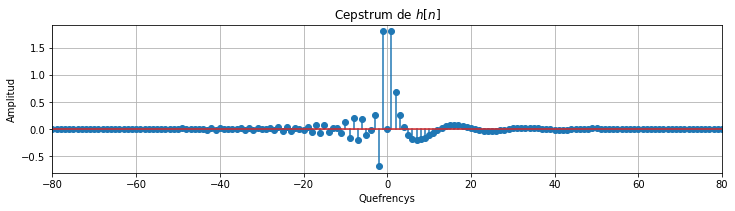
\includegraphics[width=0.8\textwidth]{hhath.png}
\caption{Gráfica de $\hat{h}[n]$}
\label{hhath}
\end{figure}

\subsubsection{3}
En esta parte se intentara calcular el cepstrum complejo de la señal $s[n] = h[n]*p[n]$. Para esto seguimos el mismo procedimiento que en las partes anteriores. En primer lugar calculamos la transformada Z y utilizando que la convolución pasa a multiplicación se tiene
$$S(z) = H(z)P(z)$$
luego se toma el logaritmo
$$Log(S(z)) = Log(H(z))+Log(P(z))$$
y ahí se reconoce que de esos logaritmos ya tenemos la antitransformada por lo que
$$\hat{s}[n]=\hat{h}[n]+\hat{p}[n]$$

\subsubsection{4}
En esta parte se calculan los cepstrum complejos con la DFT. Los resultados se adjuntan en las figuras \ref{dftp} y \ref{dfth}. Para hacer el calculo con la DFT es muy importante realizar el desdoblamiento de fase dado que estamos trabajando con el logaritmo complejo, es decir asumir una cierta continuidad en la fase del espectro y no permitir saltos abruptos. A su vez se realiza la eliminación del componente lineal en la fase para corregir la posible destrucción de la simetría impar al hacer el desdoblamiento. En ambos casos se ve como claramente el calculo de la DFT es muy parecido con el calculo analítico. 

\begin{figure}[!h]
\begin{minipage}[b]{0.5\linewidth}
\centering
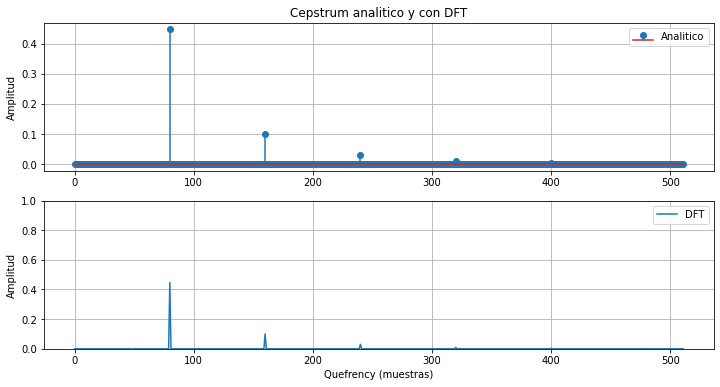
\includegraphics[width=\linewidth]{dftp.png}
\caption{Cepstrum de p analítico y con DFT}
\label{dftp}
\end{minipage}
\hspace{0.5cm}
\begin{minipage}[b]{0.5\linewidth}
\centering
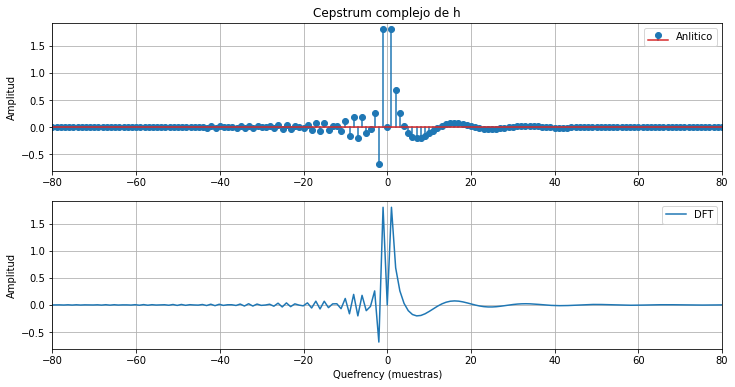
\includegraphics[width=\linewidth]{dfth.png}
\caption{Cepstrum de h analítico y con DFT}
\label{dfth}
\end{minipage}
\caption{Comparación entre diferentes cálculos del cepstrum}
\label{comparacion1}
\end{figure}

\subsubsection{5}
Para esta parte es necesario realizar un liftrado de la señal s, para eso se utiliza la expresión de la parte 3 y que además la primer delta asociada al tren de deltas se ubica en P. Es por esto que se puede liftrar con 
$$l[n] = \begin{cases}
  1  & |n| \leq q_c  \\
  0 & |n| > q_c
\end{cases}$$
con $q_c$ menor al periodo del tren de impulsos, que en este caso fue denominado como P. Se eligió $q_c = 79.31$ dado que era el valor mas cercano a $80$ que permitía la resolución de la DFT que se estaba utilizando. A su vez se eligió el mas cercano para truncar lo menos posible. El resultado de liftrar se presenta en la figura \ref{liftrado}.
\begin{figure}[h!]
\centering
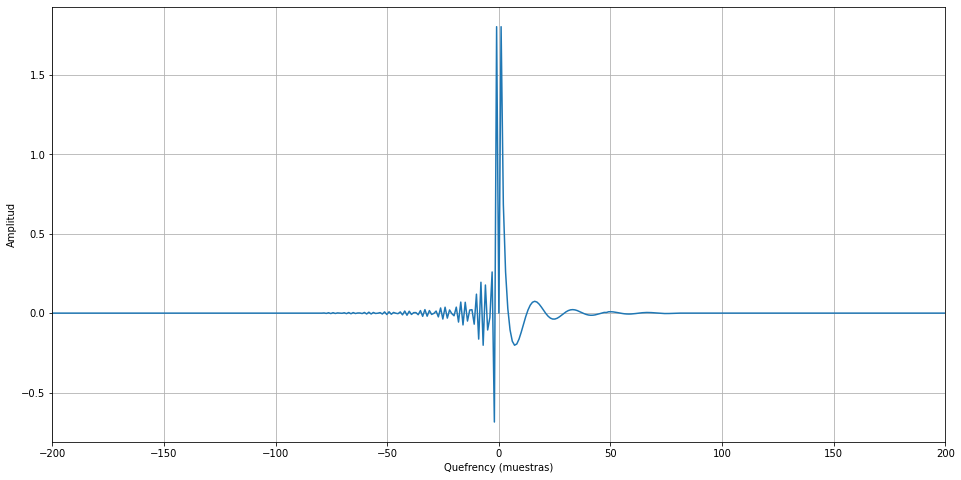
\includegraphics[width=0.8\textwidth]{liftrado.png}
\caption{$\hat{s}[n]$ liftrado con $l[n]$}
\label{liftrado}
\end{figure}
Luego, para recuperar $h[n]$ se calcula el cepstrum inverso. Para eso se calcula transformada del resultado post-liftrado, se toma la exponencial y luego se hace la transformada inversa. El resultado obtenido se adjunta en la figura \ref{hest}, en esa figura se aprecia una pequeña diferencia entre el original y la estimación, esto es causado por dos razones la primera es el hecho de que se realizo un truncamiento en el dominio de las quefrencies por lo que claramente se perdió información, la segunda es la explicación del desfasaje notorio entre las señales, esto es por el retardo introducido a la hora de linealizar la fase. 

\begin{figure}[h!]
\centering
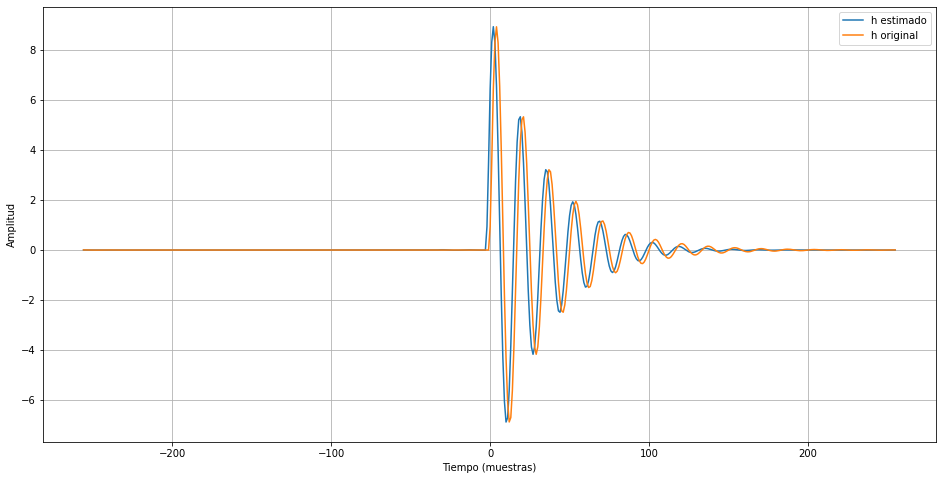
\includegraphics[width=0.8\textwidth]{hest.png}
\caption{Estimación de $h[n]$ y $h[n]$ original}
\label{hest}
\end{figure}


\subsection{Parte 2}
La idea es utilizar el hecho de que para señales sonoras se forman picos del cepstrum en los lugares donde la señal es sonora y la quefrency donde se da el pico corresponde al periodo de la señal. El algoritmo es entonces calcular el cepstrum de cada fragmento de tiempo corto, luego para cada fragmento se busca un pico del cepstrum en las medianas y altas quefrencies, si el pico pasa cierto umbral se considera que es sonoro, y donde se de el pico es la frecuencia fundamental. Si el pico no pasa el umbral o directamente no hay pico, se considera que el sonido es sordo y se lleva esa frecuencia a 0. Para que la detección se haga en las medianas y altas frecuencias, a cada frame se le aplico un liftrado pasa altos. 
En primer lugar se calculo un espectrograma pero con quefrencies, este se adjunta en la figura \ref{quefrenciograma}. En este se puede ver en primer lugar el liftrado pasa altos dado que hay una franja limpia centrada en 0. El contorno que se ve es el de las frecuencias fundamentales. 

\begin{figure}[h!]
\centering
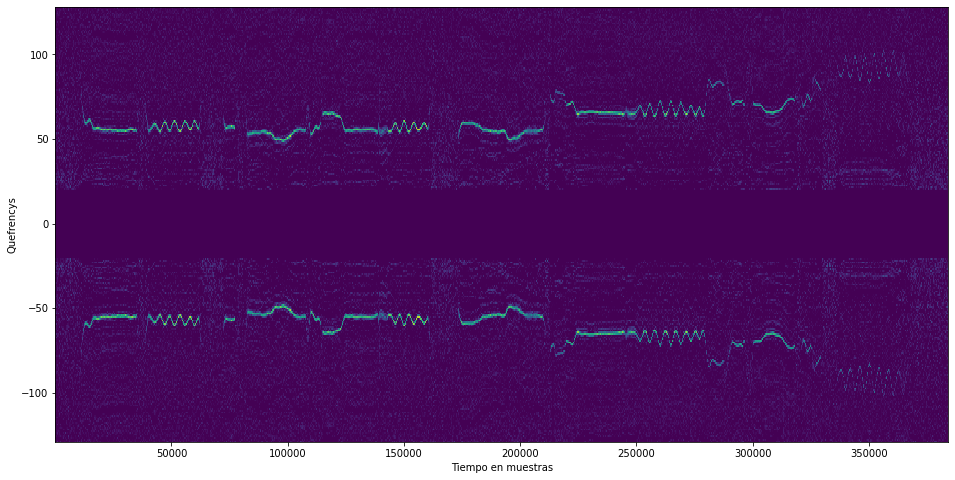
\includegraphics[width=0.8\textwidth]{quefrenciograma.png}
\caption{''Quefrenciograma''}
\label{quefrenciograma}
\end{figure}
 Programando el procedimiento que se explico mas arriba se llego al resultado presentado en la figura \ref{deteccion} junto con el ground truth. Se puede ver como solamente hay algunos errores que incluso se podrían mejorar afinando la elección del umbral. Este método, es sin dudas, el que ha producido el mejor resultado para resolver el problema de detección de pitch.
\begin{figure}[h!]
\centering
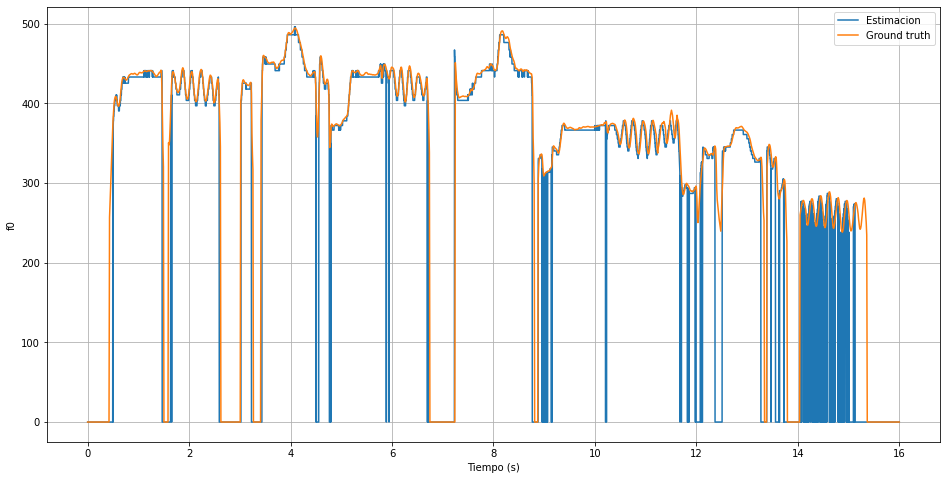
\includegraphics[width=0.8\textwidth]{deteccion.png}
\caption{Detección de $f_0$ con cepstrum real de tiempo corto y comparación con ground truth}
\label{deteccion}
\end{figure}

\section{Ejercicio 2}
\subsection{Parte 1}
\subsubsection{1}
Por definición se tiene que 
$$E_n = \sum_m e_n^2[n] = \sum_m \bigg(s_n[m]-\sum_{k=1}^P\alpha_ks_n[m-k]\bigg)^2$$
Dado que queremos minimizar $E_n$ se deriva y se iguala a 0. Para derivar se aplica regla de la cadena.
$$\frac{\partial E_n}{\partial \alpha_i}= \sum_m 2 \bigg(s_n[m]-\sum_{k=1}^P\alpha_ks_n[m-k]\bigg)s_n[m-i]=0$$
Luego despejando se tiene que
$$\sum_m s_n[m]s_n[m-i] = \sum_m \sum_{k=1}^P \hat{\alpha}_ks_n[m-k]s_n[m-i]$$
y re ordenando se tiene
$$\sum_{k=1}^{p}\hat{\alpha}_k\sum_m s_n[m-i]s_n[m-k]=\sum_m s_n[m-i]s_n[m]$$
\subsubsection{2}
En esta parte se intentara demostrar otra manera de escribir $E_n$ para eso comenzamos multiplicando las ecuaciones normales de la parte anterior por $\alpha_i$ y sumando $\forall i$
$$\sum_{i=1}^p\hat{\alpha}_i\sum_{k=1}^p\hat{\alpha}_k\sum_ms_n[m-i]s_n[m-k]=\sum_{i=1}^p\hat{\alpha}_i\sum_ms_n[m-i]s_n[m](1)$$
por otro lado desarrollamos $E_n$
$$E_n = \sum_m \bigg(s_n[m]-\sum_{k=1}^P\alpha_ks_n[m-k]\bigg)^2 = \sum_m s_n^2[m] -\sum_m\bigg(2\sum_{k=1}^p\hat{\alpha}_ks_n[m]s_n[m-k]\bigg) +$$
$$
\sum_m\bigg(\sum_{i=1}^p\hat{\alpha}_i s_n[m-i]\sum_{k=1}^p\hat{\alpha}_ks_n[m-k]\bigg)$$
Donde el ultimo termino se puede sustituir por la primer expresión que se obtuvo en $(1)$ 
$$E_n = \sum_n s_n[m]^2 - 2\sum_m\sum_{k=1}^ps_n[m]s_n[m-k] +\sum_{i=1}^p\sum_ms_n[m-i]s_n[m]$$
dado que sumar en $i$ y en $k$ es exactamente lo mismo se llega al objetivo
$$E_n = \sum_m s_n^2[m]-\sum_{k=1}^p\hat{\alpha}_k\sum_m s_n[m]s_n[m-k]$$


\subsection{Parte 2}
En esta parte se implementa un algoritmo para la clasificación de vocales utilizando LPC. 
Para esto se realizo un análisis LPC utilizando la autocorrelación y estableciendo un modelo todo polos de la señal de vos para luego obtener la frecuencia de las primeras dos formantes. Lo primero que se debió elegir es el orden del modelo todo polos, utilizando la regla del pulgar mencionada en clase \cite{of22}, se eligió $p \approx \frac{f_s}{1000}+3$. Esta elección se basa en que en el tracto vocal tiene aproximadamente una formante cada $1000Hz$. Luego se necesitan aproximadamente $3$ polos mas para poder modelar el pulso glotal y el modelo de radiación. 
Luego se procede a la elección del ancho de la ventana. Siguiendo las sugerencias de la clase \cite{of22} se elige una ventana de ancho $240$ para que sea de $30ms$. El tipo de ventana elegido es ''hann''. 
El algoritmo sigue el siguiente pseudocódigo:
\begin{enumerate}
    \item Centrado y enventanado de la señal de acuerdo a las consideraciones mencionadas.
    \item Análisis LPC con autocorrelación con el p elegido anteriormente
    \item Obtención de polos desde el modelo LPC. 
    \item Eliminación de polos con fase mayor a $\pi$ ya que son redundantes.
    \item Eliminación de polos que no cumplan la siguiente condición
    $$\frac{f_s}{\pi}log(\frac{1}{A_k})<200Hz$$
    donde $A_k$ es el modulo del polo.
    \item Tomar dos primeros polos y luego calcular las dos primeras formantes. 
    \item Para cada par de formantes se calcula la distancia euclídea a los valores de referencia proporcionados en el notebook y se clasifica la vocal de acuerdo a la menor distancia posible.
\end{enumerate}

El punto 5 corresponde a un umbral para el ancho de banda, la idea es que las formantes van a estar determinadas por los polos mas cercanos a la circunferencia unidad, esto hace que debamos limitar el modulo de alguna manera,  para eso es que se establece el umbral de $200Hz$, la elección de este umbral es siguiendo una regla del pulgar comúnmente utilizada. 

Este algoritmo se probo en vocales de un hablante masculino y femenino. Los resultados se presentan en las figuras \ref{martin} y \ref{cecilia}. 

\begin{figure}[h!]
\centering
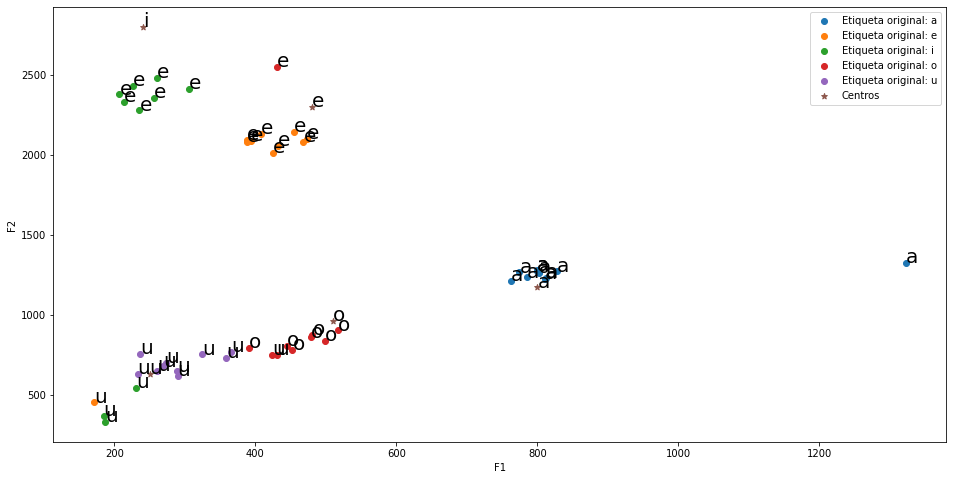
\includegraphics[width=0.8\textwidth]{martin.png}
\caption{Clasificación de vocales para hablante masculino}
\label{martin}
\end{figure}

\begin{figure}[h!]
\centering
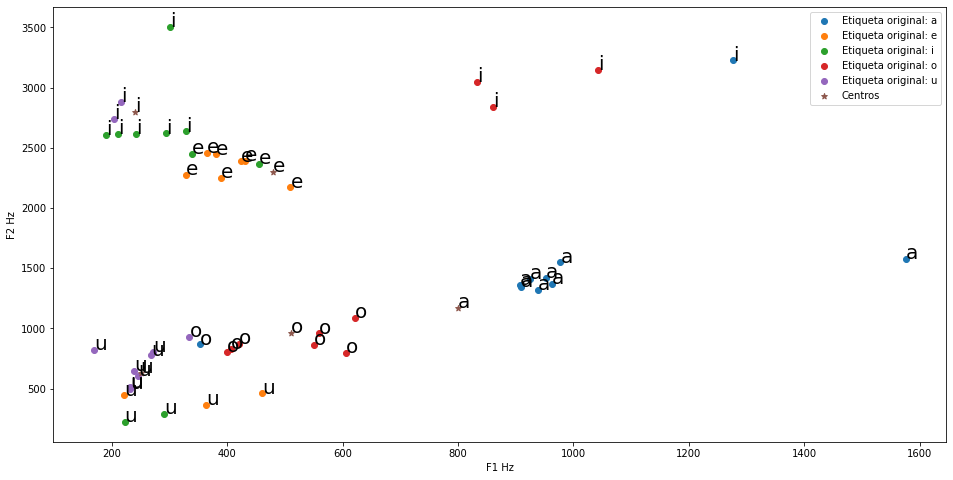
\includegraphics[width=0.8\textwidth]{cecilia.png}
\caption{Clasificación de vocales para hablante femenino}
\label{cecilia}
\end{figure}

A simple vista se parece haber obtenido un resultado relativamente satisfactorio, lo primero que llama la atención es que para el hablante masculino se clasificaron todas las $i$ erróneamente. El resumen de las tasas de acierto se presenta en las tablas \ref{tmartin} y \ref{tcecilia}.

\begin{table}[!h]
\centering
\begin{tabular}{ll}
      & Porcentaje de acierto \\
a     & 100\%                 \\
e     & 90\%                  \\
i     & 0\%                   \\
o     & 70\%                  \\
u     & 100\%                 \\
Total & 72\%                 
\end{tabular}
\caption{Tasa de acierto para hablante masculino}
\label{tmartin}
\end{table}

\begin{table}[!h]
\centering
\begin{tabular}{ll}
      & Porcentaje de acierto \\
a     & 80\%                  \\
e     & 70\%                  \\
i     & 60\%                  \\
o     & 70\%                  \\
u     & 70\%                  \\
Total & 70\%                 
\end{tabular}
\caption{Tasa de acierto para hablante femenino}
\label{tcecilia}
\end{table}

Con los resultados numéricos se puede ver que la tasa de aciertos fue muy similar para ambos hablantes, la mayor diferencia se encuentra en que para el hablante femenino se mantiene un acierto en cada vocal siempre mayor a $60\%$ pero para el masculino se obtiene un acierto de $0\%$ en la vocal ''i''. Inspeccionando los valores, la diferencia en las distancias para clasificar entre ''e'' e ''i'' es muy pequeña por lo que quizás en estos casos hubiese servido la utilización de métodos mas sofisticados de clasificación. Otra manera de mejorar estos resultados podría ser una búsqueda de umbrales mas sofisticada en la que se probara agregar mas o menos polos y aumentar o disminuir el umbral para el ancho de banda.


\newpage
\begin{thebibliography}{100} % 100 is a random guess of the total number of
%references
\addtolength{\leftmargin}{0.2in} % sets up alignment with the following line.
\setlength{\itemindent}{-0.2in}
\bibitem[RS1]{RS1}Rabiner, L. R. (2011c). The cepstrum and homomorphic speech processing. In R. W. Schafer (Ed.), Theory and applications of digital speech processing (1st ed., pp. 399–466). Pearson.
\bibitem[RS2]{RS2} Rabiner, L. R. (2011b). Linear predictive analysis of speech signals. In R. W. Schafer (Ed.), Theory and applications of digital speech processing (1st ed., pp. 473–560). Pearson.
\bibitem[OF16]{of16} [Modelado espectral], [Martín Rocamora], Proyecto OpenFING, [https://open.fing.edu.uy/courses/audiodsp/16], publicado bajo una licencia CC By NC ND.
\bibitem[OF17]{of17}[Análisis Homomórfico I], [Martín Rocamora], Proyecto OpenFING, [https://open.fing.edu.uy/courses/audiodsp/17], publicado bajo una licencia CC By NC ND.
\bibitem[OF18]{of18}[Análisis Homomórfico II], [Martín Rocamora], Proyecto OpenFING, [https://open.fing.edu.uy/courses/audiodsp/18], publicado bajo una licencia CC By NC ND.
\bibitem[OF18]{of19}[Análisis Homomórfico III], [Martín Rocamora], Proyecto OpenFING, [https://open.fing.edu.uy/courses/audiodsp/19], publicado bajo una licencia CC By NC ND.
\bibitem[OF20]{of20}[Análisis por predicción lineal I], [Martín Rocamora], Proyecto OpenFING, [https://open.fing.edu.uy/courses/audiodsp/20], publicado bajo una licencia CC By NC ND.
\bibitem[OF22]{of22}[Análisis por predicción lineal II], [Martín Rocamora], Proyecto OpenFING, [https://open.fing.edu.uy/courses/audiodsp/22], publicado bajo una licencia CC By NC ND.
\end{thebibliography}



\end{document}